\documentclass{article}




% Language setting
% Replace `english' with e.g. `spanish' to change the document language
\usepackage[english]{babel}

% Set page size and margins
% Replace `letterpaper' with `a4paper' for UK/EU standard size
\usepackage[letterpaper,top=2cm,bottom=2cm,left=3cm,right=3cm,marginparwidth=1.75cm]{geometry}

% Useful packages
\usepackage{amsmath}
\usepackage{graphicx}
\usepackage[colorlinks=true, allcolors=blue]{hyperref}

\usepackage{tikz}


\title{The impact of AI on education}
\author{MALLET Samuel}

\begin{document}
\maketitle

\begin{abstract}
    The goal of this report is to provide a comprehensive
    overview of the impact of artificial intelligence (AI)
    on education, exploring the benefits, challenges, and
    future implications of integrating AI technologies into
    learning and teaching processes. The report aims to cover
    various aspects, from personalized learning and
    accessibility to the evolving roles of teachers and the
    development of creativity and critical thinking skills
    in the AI era.
\end{abstract}
% add the ./images/chatgpt_acceptable_usecases.png image:

\newpage

\tableofcontents

\newpage
\section{Introduction}

\newpage
\section{The Building Blocks of AI in Education: Language, Speech, and Conversation}
\subsection{Defining Artificial Intelligence}

\subsubsection{Challenges of defining AI}


Artificial Intelligence (AI) has become a buzzword in recent years, with its
applications spanning across various domains, including education. However,
defining AI is not a straightforward task due to several challenges. Firstly,
there is a lack of a universally accepted definition of AI across different
fields and contexts(https://www.semanticscholar.org/paper/6f18cf33eb6e22b1fd665bd24ddf1e9c0509a420)(https://www.semanticscholar.org/paper/147fde8bd3c092aeb9372c85cedb460d9f22a2ee).
The concept of AI is complex and multifaceted, making it challenging to arrive
at a precise, all-encompassing definition. Secondly, the rapidly evolving
nature of AI technologies makes it difficult to establish a fixed
definition(https://www.semanticscholar.org/paper/6624236a5ab39d57d2463fca646e15973a5a6a55)
(https://www.semanticscholar.org/paper/147fde8bd3c092aeb9372c85cedb460d9f22a2ee).
As AI capabilities expand, any definition may quickly become outdated.
% TODO : Similarly, when Apple's Siri virtual assistant was first introduced in 2011, it was seen as a groundbreaking AI technology. But today with the advancements of technologies such as chatgpt, it is seen as outdated. 
For instance, a simple linear regression, which is a statistical method used
to model the relationship between a dependent variable and one or more
independent variables, would be considered as AI by some, while others
would argue that it is just statistics. However, one could argue that all
artificial intelligence techniques are essentially based on statistics.
Even the latest revolutionary AIs work by "predicting the next word" based
on patterns in large datasets. Lastly, various fields, such as computer
science, philosophy, and law, approach AI from different perspectives and
with different goals in mind, leading to a range of definitions that may
not always align(https://www.semanticscholar.org/paper/d45e5a95b3442afd3028e87edd060fcbacd128dc)
(https://www.semanticscholar.org/paper/b1c7a9ef833287615fae3324eae044fc76839460).

\subsubsection{Common definitions}

Despite the challenges in defining AI, there are some common definitions
that are widely used. For example, Wikipedia defines AI as "intelligence
demonstrated by machines", as opposed to the natural intelligence displayed
by animals including humans. Similarly, the Oxford English Dictionary
defines AI as "The capacity of computers or other machines to exhibit or
simulate intelligent behaviour." However, these definitions are themselves
based on the concept of intelligence, which is also not a trivial task to
define.

Interestingly, what is hard for humans is often easy for computers, and vice
versa. For instance, it is hard for us to make complex computations quickly,
but simple for computers. On the other hand, it is trivial for us to recognize
animals, stop signs, talk, and drive, but these tasks are incredibly
challenging for computers to perform accurately and consistently. In practice,
what is considered as artificial intelligence is often what has been
challenging or seen as impossible for computers in the past. As computers
become more capable of performing tasks that were once thought to be the
exclusive domain of human intelligence, the definition of AI continues
to evolve and expand.

\subsection{Fields of AI}

% add the images/AI_ML_DL.png
\begin{figure} %TODO : mention this  in text
    \centering
    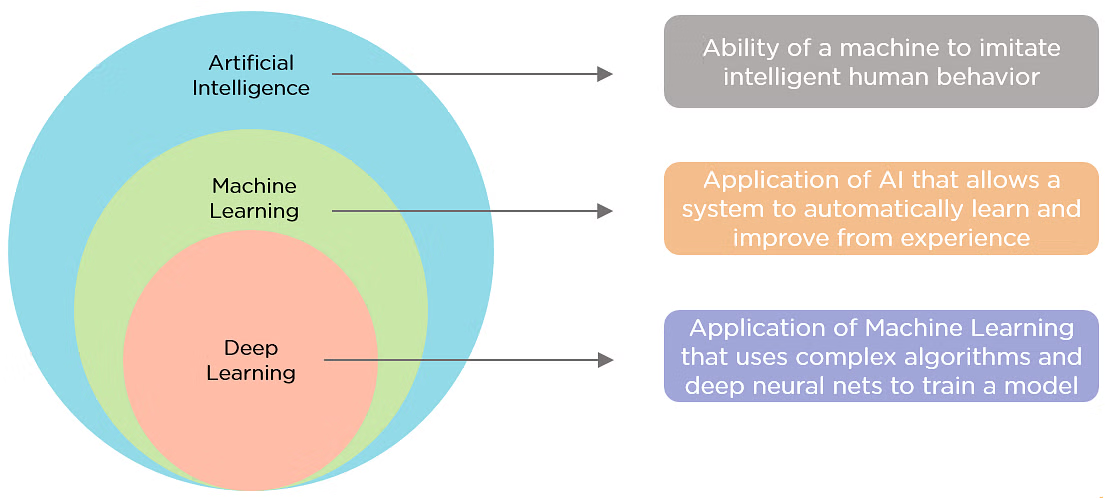
\includegraphics[width=0.8\textwidth]{images/AI_ML_DL.png}
    \caption{AI vs Machine Learning vs Deep Learning}
    %TODO : include source (https://www.simplilearn.com/tutorials/artificial-intelligence-tutorial/ai-vs-machine-learning-vs-deep-learning)
\end{figure}



The Artificial Intelligence landscape is vast and encompasses a wide range
of subfields and techniques. Nearly all the recent breakthroughs in AI
can be attributed to the subfield called Machine Learning.

\subsubsection{Introduction of Machine learning (ML)}

Machine Learning (ML) is a special type of AI programming that allows
computers to learn from data, rather than being explicitly programmed
with rules. To illustrate this concept, let's consider the task of
distinguishing between pictures of cats and dogs. It would be incredibly
difficult, if not impossible, to write down all the rules that would
account for all the possible variations in size, color, shape, and
behavior.

This is where Machine Learning comes in. Instead of trying to write down
all these rules, we can provide the computer with a large collection of
labeled pictures (i.e., pictures that have been identified as either a cat
or a dog). The computer then uses statistical techniques to find patterns
and relationships within these pictures. For example, it might learn that
dogs usually have longer noses than cats, or that cats have pointy ears
while dogs' ears are more rounded.

Once the computer has learned these patterns, it can then use them
to correctly identify cats and dogs in new pictures that it hasn't
seen before. In essence, Machine Learning is like giving the computer
a set of examples to learn from, rather than a set of rules to follow.
This makes it a powerful tool for solving complex problems that would
be too difficult for traditional programming. And the best part is,
the more data the computer has to learn from, the better it becomes
at making accurate predictions.

Machine Learning has a wide range of applications across various
domains, including image and speech recognition, natural language
processing (NLP), recommendation systems, fraud detection, predictive
maintenance, autonomous vehicles, healthcare, and many more.

\subsubsection{Deep Learning}

Nearly all the recent breakthroughs in Machine Learning can be attributed
to the field of Deep Learning. Deep Learning uses layers of artificial
"neurons" in a way that is similar to how the human brain learns.
This approach is very flexible but requires a lot of data and computer
power.

Thanks to Deep Learning, computers are now able to perform tasks that
were previously thought to be too difficult for them, such as recognizing
speech or understanding natural language. Deep Learning has revolutionized
the field of AI and has opened up new possibilities for solving complex
problems.

\subsection{The technologies we will focus on in this report}

We will not focus on AIs able to distinguish between cats and dogs, or systems that predict the price of Bitcoin. Instead, we will focus on AI technologies that can "understand" and produce human language, and allow engaging conversations between computers and humans.

\subsubsection{Natural Language Processing (NLP)}

Natural Language Processing (NLP) is an interdisciplinary subfield
of computer science and information retrieval concerned with giving
computers the ability to understand, interpret, and manipulate human
language . The goal is a computer capable of "understanding"
the contents of documents, including the contextual nuances of the
language within them.

Up until the 1980s, most NLP systems were based on complex sets of
hand-written rules. In the late 1980s, there was a revolution in NLP with
the introduction of machine learning algorithms for language processing,
due to increasing computational power. In the 2010s, representation learning
and deep neural network-style machine learning methods became widespread in
NLP, due to their achieving state-of-the-art results in many natural language
tasks.

The development of large pre-trained language models using neural networks and
vast amounts of text data has led to significant advancements in
NLP capabilities in recent years.


The development of large pre-trained language models using neural networks and vast amounts of text data has led to significant advancements in NLP capabilities in recent years.

\subsubsection{Large Language Models (LLM)}

Large Language Models (LLMs) are deep learning models trained on massive
amounts of text data to understand and generate human language. They can
perform a wide range of NLP tasks without requiring task-specific training data.
There are a large number of LLMs available, both open-source and closed-source.
Open-source models like Llama (developed by Meta), the "Mistral" models
developed by the French company Mistral, and many more are available to
researchers, companies, and the community. Closed-source models are
developed by companies like OpenAI (GPT-3, GPT-4), Anthropic (Claude),
and Google (Gemini).
LLMs range in size from millions to hundreds of billions of parameters.
Larger models generally have better performance but require more computational
resources. State-of-the-art LLMs exhibit impressive language understanding
and generation capabilities across many benchmarks and real-world
applications. However, LLMs have a limited context window, typically
a few pages of text, limiting their ability to process very long documents
or maintain long-term memory.
LLMs have various applications, such as chatbots and conversational AI
(like ChatGPT) that engage in open-ended dialogue, text generation,
summarization, translation, creative writing assistance, knowledge
retrieval, and question answering from large knowledge bases.
However, LLMs have some limitations in the education context. Training
and running large LLMs is hugely energy-intensive, raising environmental
concerns. Smaller models are more efficient and can even run on phones.
LLMs excel at pattern matching and information retrieval but struggle
with tasks requiring logical reasoning, causal understanding, and domain
expertise. They can also generate plausible but factually incorrect
statements (known as "hallucinations"), which is problematic for
educational applications where accuracy is critical.

\subsubsection{Vision}

More and more LLMs come with vision capabilities, allowing them to handle not just text but also images and even videos. LLMs can perform general-purpose vision tasks such as answering questions about image content, recognizing objects, scenes, and visual concepts, generating detailed, contextual captions and descriptions for images, visual grounding and reasoning (e.g., locating objects mentioned in a query), providing visual explanations and differentiating between similar images/classes, and enabling open-ended visual task instructions via natural language.

Some examples of vision-capable models include GPT-4 (OpenAI), the Claude 3 family of models (Anthropic), and Grok 1.5 Vision (xAI).

\subsubsection{Speech Recognition and Synthesis}

Speech recognition involves converting spoken language into written text. Previous models were not well-suited for human conversation, requiring exaggerated voice clarity and only recognizing one language at a time. Whisper, an open-source speech recognition model by OpenAI, significantly improved performance, understanding technical vocabulary and multiple languages in one conversation.

Speech synthesis has also advanced, with new models capable of simulating emotions and allowing interruptions, enabling more natural human-like conversations.

Combining speech recognition, NLP, and speech synthesis enables real-life conversations with AI, which are faster and more engaging than typing. Example applications include PI.ai, which helps users better understand their emotions without simulating affection, reducing the risk of emotional dependence (although the AI may sometimes be overly supportive), and ChatGPT voice, which allows fluid conversations, such as practicing job interviews with the AI simulating an employer role.

However, the current process of converting voice to text, processing, and converting back to voice removes emotional nuances like irony, humor, and doubt. State-of-the-art solutions are being developed to address this issue.

\subsubsection{Building on LLMs} %TODO : add examples, and clarify the RAG

Beyond chatbots in web browsers, LLMs can be integrated into a wide range of tasks. LLMs are steerable and can act as teachers, experts, or take on various roles. They enable automation and integration with other systems and workflows. For instance, LLMs can be integrated into customer service, and other examples are yet to be explored.

Retrieval-Augmented Generation (RAG) combines LLMs with external knowledge retrieval to enhance their factual accuracy and knowledge coverage.

\subsubsection{Summary}%TODO : add a summary


\newpage
\section{The Growing Influence of AI in Education}
\subsection{Record-Breaking User Growth}
ChatGPT achieved unprecedented user growth, becoming the fastest-growing consumer application in history \cite{https://arstechnica.com/information-technology/2023/02/chatgpt-sets-record-for-fastest-growing-user-base-in-history-report-says/}. It surpassed 1 million users within just 5 days of launch and skyrocketed to 100 million monthly active users by January 2023, only two months after its debut \cite{https://meetanshi.com/blog/chatgpt-statistics/} \cite{https://nerdynav.com/chatgpt-statistics/} \cite{https://www.namepepper.com/chatgpt-users}. For comparison, TikTok took 9 months and Instagram about 2.5 years to reach the 100 million user milestone \cite{https://arstechnica.com/information-technology/2023/02/chatgpt-sets-record-for-fastest-growing-user-base-in-history-report-says/}.
As of August 2023, ChatGPT boasts over 180.5 million users, an 80.5% increase in just 8 months \cite{https://meetanshi.com/blog/chatgpt-statistics/} \cite{https://nerdynav.com/chatgpt-statistics/} \cite{https://www.namepepper.com/chatgpt-users}.
\subsection{Global Reach and Demographics}
ChatGPT has a global presence, with users spanning 161 countries \cite{https://meetanshi.com/blog/chatgpt-statistics/}. However, it remains banned in several nations, including China, Russia, Iran, and Venezuela \cite{https://meetanshi.com/blog/chatgpt-statistics/} \cite{https://nerdynav.com/chatgpt-statistics/}.
The United States accounts for the largest share of users at 46.75%, followed by India at 5.47% \cite{https://nerdynav.com/chatgpt-statistics/}. In terms of demographics, 55.99% of ChatGPT users are male, while 44.01% are female \cite{https://nerdynav.com/chatgpt-statistics/}. But most importantly, the majority of users (62.52%) are young, between the ages of 18 and 34 \cite{https://nerdynav.com/chatgpt-statistics/}.
\subsection{News coverage and public attention}
The impact of AI on education has garnered significant media attention, with numerous articles discussing the potential benefits, risks, and implications for students and teachers \cite{https://www.bbc.com/news/education-67433036} \cite{https://www.tampabay.com/opinion/2024/02/22/artificial-intelligence-education-return-once-feared-calculator-or-new-opportunity/} \cite{https://theweek.com/education/ai-in-schools-machine-learning}. Headlines have highlighted both the revolutionary potential of AI to transform learning and the challenges it poses for academic honesty and traditional educational practices. The topic has sparked widespread public debate about the appropriate role and regulation of AI tools in schools \cite{https://www.tampabay.com/opinion/2024/02/22/artificial-intelligence-education-return-once-feared-calculator-or-new-opportunity/} \cite{https://theweek.com/education/ai-in-schools-machine-learning}.
\subsection{Fear of Widespread Cheating and Plagiarism}
One of the primary concerns surrounding ChatGPT's launch was its potential to facilitate cheating and plagiarism among students \cite{https://oai.missouri.edu/chatgpt-artificial-intelligence-and-academic-integrity/} \cite{https://informationmatters.org/2023/02/chatgpt-and-academic-integrity/} \cite{https://www.reddit.com/r/changemyview/comments/123m3xr/cmv_using_chatgpt_for_academic_purposes_is_not_an/}. With its ability to generate high-quality, human-like text based on prompts, educators feared that students would use ChatGPT to complete assignments, essays, and exams without putting in the necessary effort or learning \cite{https://oai.missouri.edu/chatgpt-artificial-intelligence-and-academic-integrity/} \cite{https://www.reddit.com/r/changemyview/comments/123m3xr/cmv_using_chatgpt_for_academic_purposes_is_not_an/}.
A recent survey revealed that nearly half of students were likely to use AI tools like ChatGPT, while 60% perceived reliance on such tools as cheating \cite{https://oai.missouri.edu/chatgpt-artificial-intelligence-and-academic-integrity/}. The ease of use and accessibility of ChatGPT heightened concerns about the prevalence of academic dishonesty across all levels of education \cite{https://informationmatters.org/2023/02/chatgpt-and-academic-integrity/} \cite{https://www.reddit.com/r/changemyview/comments/123m3xr/cmv_using_chatgpt_for_academic_purposes_is_not_an/}.

Most cheating statistics are derived from surveys in which students are asked about their recent cheating behavior. However, to accurately interpret these statistics, it is crucial to understand what students consider to be cheating. A Pew Research Center survey of U.S. teens, conducted between September 26 and October 23, 2023, revealed an interesting discrepancy in students' perceptions of AI usage. While approximately 60% of students believe that using ChatGPT to write essays is unacceptable, around 70% consider it acceptable to use the tool for researching new topics. This finding suggests that students are more likely to view AI as an acceptable tool for exploration and learning rather than for completing actual assignments or assessments.

\begin{figure}
    \centering
    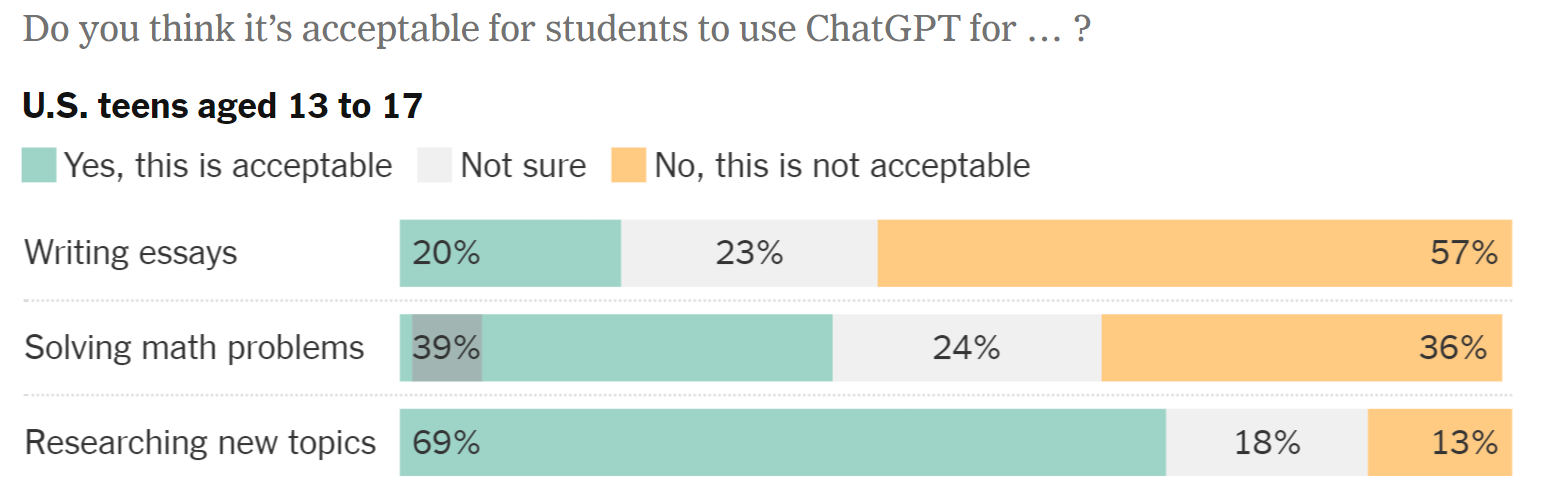
\includegraphics[width=0.8\textwidth]{images/chatgpt_acceptable_usecases.png}
    \caption{Pew Research Center survey on AI use in education}
    %TODO : add the source (https://www.nytimes.com/2023/12/13/technology/chatbot-cheating-schools-students.html)
    %TODO : better position in the text
\end{figure}

\subsection{Bans and Restrictions in Schools}
In response to the potential for widespread cheating, several large public school districts, including New York City, Los Angeles, Seattle, and Baltimore, swiftly banned access to ChatGPT on school devices and networks \cite{https://oai.missouri.edu/chatgpt-artificial-intelligence-and-academic-integrity/} \cite{https://www.reddit.com/r/changemyview/comments/123m3xr/cmv_using_chatgpt_for_academic_purposes_is_not_an/}. These bans aimed to prevent students from misusing the tool and to uphold academic integrity standards \cite{https://oai.missouri.edu/chatgpt-artificial-intelligence-and-academic-integrity/}.
However, the effectiveness of such bans remains questionable, as students can still access ChatGPT on personal devices outside of school networks \cite{https://www.reddit.com/r/changemyview/comments/123m3xr/cmv_using_chatgpt_for_academic_purposes_is_not_an/}. The bans also sparked debates about the role of AI in education and the need for schools to adapt to emerging technologies \cite{https://oai.missouri.edu/chatgpt-artificial-intelligence-and-academic-integrity/} \cite{https://www.reddit.com/r/changemyview/comments/123m3xr/cmv_using_chatgpt_for_academic_purposes_is_not_an/}.
Recent research from Stanford University suggests these cheating fears may have been overblown, as overall cheating rates in high schools have not significantly increased despite the growing use of AI tools \cite{https://www.nytimes.com/2023/12/13/technology/chatbot-cheating-schools-students.html}.
\subsection{Emergence of AI Detection Tools}
In response of the cheating concerns, various AI detection tools have been developed to help identify content that has been partially or wholly generated by AI \cite{https://kb.iu.edu/d/bimt}. These tools are intended for use by educators, publishers, recruiters, and others who want to ensure the originality and authenticity of written content. Exemples are Originality.ai \cite{https://originality.ai/}, copyleaks.com \cite{https://copyleaks.com}, quillbot.com \cite{https://quillbot.com/}, gptzero.me \cite{https://gptzero.me/}, or a French tool compilatio.net \cite{https://www.compilatio.net/ia-detecteur-info}. However, the effectiveness and reliability of these tools have been the subject of much debate \cite{https://www.scribbr.com/ai-tools/how-do-ai-detectors-work/} \cite{https://contadu.com/ai-detection-tools-the-challenge-of-todays-digital-age/} \cite{https://edintegrity.biomedcentral.com/articles/10.1007/s40979-023-00140-5}.
\subsubsection{How AI Detection Tools Work}
AI detection tools rely on machine learning (ML) and natural language processing (NLP) techniques to analyze and classify text as either human-written or AI-generated \cite{https://surferseo.com/blog/how-do-ai-content-detectors-work/} \cite{https://contadu.com/ai-detection-tools-the-challenge-of-todays-digital-age/}. They are often built using language models similar to those used in the AI writing tools they aim to detect \cite{https://www.scribbr.com/ai-tools/how-do-ai-detectors-work/}. These tools work by examining various linguistic patterns, sentence structures, and other characteristics of the text \cite{https://surferseo.com/blog/how-do-ai-content-detectors-work/} \cite{https://contadu.com/ai-detection-tools-the-challenge-of-todays-digital-age/}. They compare the input text to large datasets of known AI-generated and human-written content to determine the likelihood that the text was created by an AI \cite{https://www.scribbr.com/ai-tools/how-do-ai-detectors-work/} \cite{https://contadu.com/ai-detection-tools-the-challenge-of-todays-digital-age/}. Some common techniques used by AI detection tools include \cite{https://surferseo.com/blog/how-do-ai-content-detectors-work/} \cite{https://contadu.com/ai-detection-tools-the-challenge-of-todays-digital-age/}:
\begin{itemize}
    \item Perplexity: Measuring how well a language model predicts the next word in a sequence
    \item Burstiness: Analyzing variations in sentence structure and length
    \item Semantic techniques: Topic modeling, sentiment analysis, and consistency assessment
\end{itemize}
\subsubsection{Challenges and Limitations}
Despite the development of various AI detection tools, their effectiveness and reliability remain questionable \cite{https://www.scribbr.com/ai-tools/how-do-ai-detectors-work/} \cite{https://contadu.com/ai-detection-tools-the-challenge-of-todays-digital-age/} \cite{https://edintegrity.biomedcentral.com/articles/10.1007/s40979-023-00140-5}. Several studies have shown that these tools often struggle to accurately classify text, particularly as AI text generators become more advanced \cite{https://contadu.com/ai-detection-tools-the-challenge-of-todays-digital-age/} \cite{https://edintegrity.biomedcentral.com/articles/10.1007/s40979-023-00140-5}. Some key challenges and limitations include:
\begin{itemize}
    \item High rates of false positives and false negatives \cite{https://www.scribbr.com/ai-tools/how-do-ai-detectors-work/} \cite{https://edintegrity.biomedcentral.com/articles/10.1007/s40979-023-00140-5} \cite{https://kb.iu.edu/d/bimt}
    \item Difficulty keeping pace with rapidly evolving AI technologies \cite{https://surferseo.com/blog/how-do-ai-content-detectors-work/} \cite{https://contadu.com/ai-detection-tools-the-challenge-of-todays-digital-age/}
    \item Inconsistent performance across different AI models and generators \cite{https://edintegrity.biomedcentral.com/articles/10.1007/s40979-023-00140-5}
    \item Reduced effectiveness when faced with obfuscation techniques like manual editing or machine paraphrasing \cite{https://edintegrity.biomedcentral.com/articles/10.1007/s40979-023-00146-z}
\end{itemize}
Additionally, the results provided by AI detection tools can be difficult for average users to interpret, with some tools providing complex statistical information or highlighting text without clear explanations \cite{https://edintegrity.biomedcentral.com/articles/10.1007/s40979-023-00146-z}.

\subsubsection{An arm race}
As AI detection tools become more prevalent, users and students are employing various strategies to evade
these tools when using AI-generated content for schoolwork or other purposes. This has led to an ongoing
battle, often referred to as an "arms race," between AI generators and detectors.

Some of the techniques used to bypass AI detection include manual editing and paraphrasing, where users
take the AI-generated text and manually rephrase sentences, change word choices, and introduce minor
grammatical errors to make the writing seem more human-like and less perfect \cite{https://www.reddit.com/r/ChatGPT/comments/139wvn7/how_to_avoid_ai_detection/}
\cite{https://www.reddit.com/r/ChatGPT/comments/18f0u56/to_fool_an_ai_detector/}.

Another approach is the multilingual method, where users have AI tools like ChatGPT generate the text in a different language,
then translate it back to English themselves, which can help obscure AI patterns
\cite{https://www.reddit.com/r/ChatGPT/comments/100jw27/how_you_can_bypass_ai_detection/}.

Users also instruct AI models to mimic specific writing styles, such as a "struggling B-level student"
or a "lazy student rushing to proofread a paper," complete with intentional errors and imperfections
expected from those archetypes \cite{https://www.reddit.com/r/ChatGPTPromptGenius/comments/162anql/is_there_any_free_method_to_bypass_ai_detection/}
\cite{https://www.reddit.com/r/ChatGPT/comments/18f0u56/to_fool_an_ai_detector/}.

Some even resort to using "AI-detection-bypass" tools, which are AI-powered tools specifically designed
to rephrase AI-generated text in ways that are harder for detectors to identify. Examples of such tools
include Hix AI, Nova, Conch AI, Undetectable AI, and Stealthwriter
\cite{https://www.reddit.com/r/ChatGPT/comments/139wvn7/how_to_avoid_ai_detection/}
\cite{https://www.reddit.com/r/ChatGPTPromptGenius/comments/162anql/is_there_any_free_method_to_bypass_ai_detection/}
\cite{https://www.reddit.com/r/OpenAI/comments/zmglvv/how_to_outsmart_and_bypass_ai_content_detection/}.

Some users even exploit technical loopholes, such as replacing certain letters in their text with visually
similar Unicode characters, which can trick AI detectors
\cite{https://www.reddit.com/r/OpenAI/comments/122wlot/the_best_way_to_bypass_ai_detectors/}.

Others believe that text from more sophisticated models like GPT-4 is harder for current detectors
to identify compared to GPT-3.5 or other models \cite{https://www.reddit.com/r/ChatGPT/comments/100jw27/how_you_can_bypass_ai_detection/}.

However, many users also express doubts about the effectiveness and longevity of these methods.
Students are compiling evidence of false positives from detectors (e.g., flagging historical texts as AI-generated)
to undermine their reliability and persuade schools not to trust the tools \cite{https://www.reddit.com/r/ChatGPT/comments/18f0u56/to_fool_an_ai_detector/}
\cite{https://www.reddit.com/r/OpenAI/comments/122wlot/the_best_way_to_bypass_ai_detectors/}.
%TODO : paragraph about the term "arm race"




\subsubsection{Implications and Future Directions}
The development of AI detection tools has significant implications for academia
and beyond. Educators are grappling with how to adapt courses and assessments
to the AI era while maintaining academic integrity
\cite{https://www.scribbr.com/ai-tools/how-do-ai-detectors-work/}
\cite{https://kb.iu.edu/d/bimt}. Publishers and content creators are
also exploring ways to ensure the originality of their content
\cite{https://www.scribbr.com/ai-tools/how-do-ai-detectors-work/}.
However, the current limitations of AI detection tools suggest that they
should be used with caution and not relied upon as the sole means of
identifying AI-generated content \cite{https://edintegrity.biomedcentral.com/articles/10.1007/s40979-023-00146-z}
\cite{https://edintegrity.biomedcentral.com/articles/10.1007/s40979-023-00140-5}
\cite{https://kb.iu.edu/d/bimt}. Experts emphasize the importance of
combining automated detection with human review and other methods to ensure
the accuracy and fairness of the results \cite{https://edintegrity.biomedcentral.com/articles/10.1007/s40979-023-00146-z}
\cite{https://edintegrity.biomedcentral.com/articles/10.1007/s40979-023-00140-5}.
As AI text generators continue to advance, it is clear that AI detection tools will
need to evolve in tandem to remain effective \cite{https://surferseo.com/blog/how-do-ai-content-detectors-work/}
\cite{https://contadu.com/ai-detection-tools-the-challenge-of-todays-digital-age/}
\cite{https://edintegrity.biomedcentral.com/articles/10.1007/s40979-023-00140-5}.
This ongoing "arms race" between AI generators and detectors is likely to shape
the future of academic integrity and content authenticity in significant ways.
Educators, institutions, and policymakers will need to stay informed about the
latest developments in AI technology and adapt their practices accordingly to
ensure the integrity of the educational process in the face of these rapidly evolving tools.


\subsection{Government initiatives and policies}
%TODO : talk about MIA, the French AI learning platform 
\subsubsection{Investing in AI Infrastructure and Partnerships}
Governments around the world are increasingly recognizing the potential of AI to transform education and are investing in initiatives to support AI research, development, and deployment in academic institutions. In the United States, the National Science Foundation (NSF) is leading efforts to create a national network of AI research centers by facilitating partnerships between government agencies and academic institutions \cite{https://www2.datainnovation.org/2022-ai-universities.pdf}. These collaborations aim to increase access to AI resources for academia and support national AI goals.
The UK government has also announced a £2 million investment in new classroom technology, including AI tools, to reduce teachers' workloads and enhance education \cite{https://dig.watch/updates/uk-government-invests-2-million-in-ai-classroom-technology} \cite{https://www.openaccessgovernment.org/uk-government-invests-in-ai-powered-teacher-support/169271/}. This funding will be used by Oak National Academy to develop and expand AI-powered teacher support tools, such as lesson planners and quiz builders \cite{https://www.gov.uk/government/news/new-support-for-teachers-powered-by-artificial-intelligence} \cite{https://www.openaccessgovernment.org/uk-government-invests-in-ai-powered-teacher-support/169271/}.
In 2018, the French government launched a national strategy for artificial intelligence (AI) called "AI for Humanity." This strategy aims to position France as a global leader in AI research, development, and innovation \cite{https://www.economie.gouv.fr/strategie-nationale-intelligence-artificielle} \cite{https://www.entreprises.gouv.fr/fr/numerique/enjeux/la-strategie-nationale-pour-l-ia}. The strategy is divided into two phases:
\begin{enumerate}
    \item Phase 1 (2018-2022): Focused on strengthening France's research capabilities in AI, with an investment of €1.5 billion \cite{https://www.economie.gouv.fr/strategie-nationale-intelligence-artificielle} \cite{https://www.entreprises.gouv.fr/fr/numerique/enjeux/la-strategie-nationale-pour-l-ia} \cite{https://www.enseignementsup-recherche.gouv.fr/fr/la-strategie-france-ia-soutenir-la-dynamique-francaise-autour-de-l-intelligence-artificielle-46305}.
    \item Phase 2 (2021-2025): Aims to diffuse AI technologies throughout the economy and support the development of trustworthy, frugal, and generative AI. This phase has a budget of €1.5 billion as part of the France 2030 plan \cite{https://www.economie.gouv.fr/strategie-nationale-intelligence-artificielle} \cite{https://www.entreprises.gouv.fr/fr/numerique/enjeux/la-strategie-nationale-pour-l-ia}.
\end{enumerate}
The French government has supported the creation and development of a network of interdisciplinary AI institutes, the establishment of chairs of excellence, and doctoral programs \cite{https://www.entreprises.gouv.fr/fr/numerique/enjeux/la-strategie-nationale-pour-l-ia} \cite{https://www.enseignementsup-recherche.gouv.fr/fr/la-strategie-france-ia-soutenir-la-dynamique-francaise-autour-de-l-intelligence-artificielle-46305}. It has also deployed the Jean Zay supercomputer to support AI research \cite{https://www.entreprises.gouv.fr/fr/numerique/enjeux/la-strategie-nationale-pour-l-ia}.

%TODO conclude with how the investments are absolutely massive.



\subsubsection{Developing Frameworks and Guidelines}
Governments and international organizations are developing frameworks and guidelines to ensure the safe, ethical, and effective use of AI in education. For example, the Australian Government Department of Education has released the inaugural Australian Framework for Generative Artificial Intelligence in Schools, to be implemented from Term 1 2024 \cite{https://www.educationmattersmag.com.au/federal-government-releases-first-ai-framework-for-schools/}. The framework prioritizes privacy, security, safety, teaching and learning outcomes, human and social wellbeing, transparency, fairness, and accountability \cite{https://www.educationmattersmag.com.au/federal-government-releases-first-ai-framework-for-schools/}.
UNESCO has also developed policy guidance for leveraging AI in education, emphasizing the need to harness the benefits of AI while mitigating risks \cite{https://www.teachingtomorrow.co.uk/news/artificial-intelligence-in-education-empowering-teachers-and-students}. The guidance covers various aspects, including promoting inclusive and equitable use of AI, developing ethical guidelines, fostering local AI innovations, and building an evidence base through pilot testing and evaluation \cite{https://www.teachingtomorrow.co.uk/news/artificial-intelligence-in-education-empowering-teachers-and-students}.
As part of its broader national strategy for artificial intelligence (AI), the French government has recognized the importance of integrating AI into the education system. The strategy aims to position France as a global leader in AI research, development, and innovation, with education playing a crucial role \cite{https://www.economie.gouv.fr/strategie-nationale-intelligence-artificielle} \cite{https://www.entreprises.gouv.fr/fr/numerique/enjeux/la-strategie-nationale-pour-l-ia}. In March 2024, the Commission on Artificial Intelligence submitted a report to the President of the Republic containing 25 recommendations to help France capitalize on the AI technological revolution \cite{https://edunumrech.hypotheses.org/11602} \cite{https://www.ac-paris.fr/l-intelligence-artificielle-dans-l-education-130992} \cite{https://www.campusmatin.com/numerique/equipements-systemes-informations/commission-ia-les-recommandations-pour-l-enseignement-superieur-et-la-recherche.html}. These recommendations were based on extensive consultations and aim to guide public authorities in making decisions to position France at the forefront of AI, including in the field of education.




\subsection{Conclusion (TODO)} %TODO : conclusion on the growing influence of AI in education

\newpage


\section{Benefits of AI in Education}
%TODO : introduction

\subsection{Existing Benefits of Digital Tools}

Even without AI, the digital world offers numerous opportunities to enhance learning experiences. Throughout this section, we will explore three excellent examples: Brilliant, an online learning platform; Remnote, a note-taking app; and Duolingo, a language learning app.

Brilliant is an interactive online learning platform that offers guided courses and problem-solving challenges in math, science, and computer science to develop critical thinking and creative problem-solving skills \cite{https://brilliant.org/}.

Duolingo is a free language-learning platform that offers fun, bite-sized lessons in over 40 languages, as well as courses in math and music, through its mobile app and website.

Remnote is a revolutionary note-taking software designed to help users remember what they learn. While it may appear similar to classic note-taking apps, with features like writing, inserting images, links, colors, and multiple pages, Remnote's true power lies in its unique approach to learning and retention.

\begin{figure}[h]
    %TODO : cite this
    \centering
    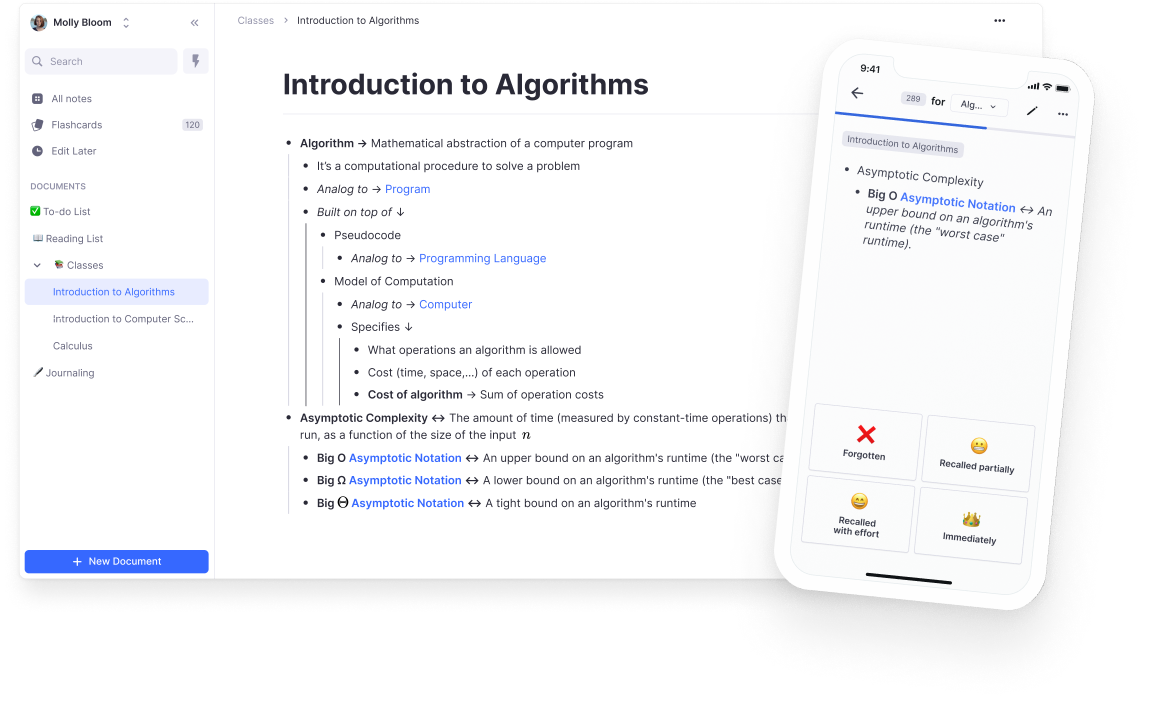
\includegraphics[width=0.8\textwidth]{./images/remnote_ad.png}
    \caption{Remnote advertizing (https://www.remnote.com)}
\end{figure}

\subsubsection{Optimized Learning Experience}

Remnote leverages two powerful learning techniques: active recall and spaced repetition.

\textbf{Active Recall}

Reading through notes and trying to remember the content is an inefficient way to learn. While reading may give a false sense of knowing, being able to recall information from memory without referring to the text is a different skill altogether. Having someone test you on the subject would be far more effective, as it would highlight areas you don't know and allow you to focus on them, thus optimizing your learning process. This is known as the testing effect \cite{https://en.wikipedia.org/wiki/Testing_effect}.

Flashcards are one of the best learning techniques that leverage active recall. By writing a hint on the front side and the answer on the back, you can test yourself effectively. Many websites offer services to create and practice flashcards, such as Anki.

However, creating flashcards is often a separate step after taking handwritten or digital notes, resulting in two sources of information and wasted time. Remnote takes a different approach: your notes \textit{are} the flashcards. You create flashcards \textit{while} taking notes, streamlining the process. The resulting flashcards are not just an unsorted list of unrelated cards disconnected from your notes; they are an integral part of your learning material.

\textbf{Spaced Repetition}

\begin{figure}[h]
    \centering
    %TODO : cite this
    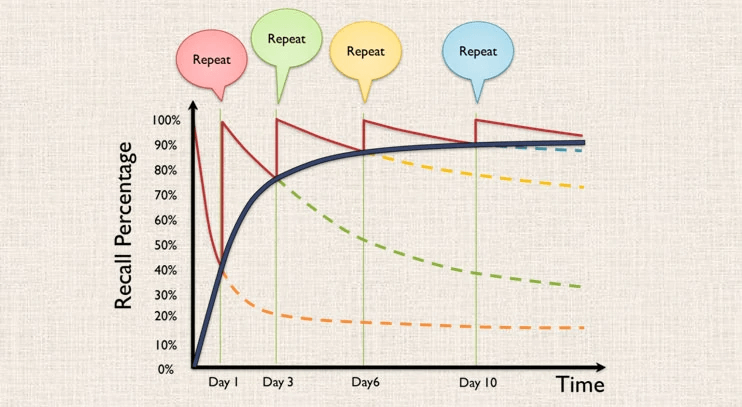
\includegraphics[width=0.8\textwidth]{images/spaced_repetition_principle.png}
    \caption{Spaced repetition graph (https://www.heylama.com/blog/spaced-repetition)} %TODO : improve source format
\end{figure}

Students who cram just before an exam may remember some material during the test but often forget most of it quickly afterward. While practicing a subject once a day over a long period can lead to long-term retention, it is not always practical or necessary. For example, a doctor doesn't need to review their textbooks daily to remember the symptoms of hepatitis. However, when they were in school, they likely forgot the information soon after learning it for the first time, but by practicing again a day later, then a week later, and so on, they were able to retain the knowledge.

The optimal frequency for long-term retention involves practicing frequently at the beginning, then gradually increasing the intervals between practice sessions. This is the science of "spaced repetition," a crucial concept for improving learning efficiency.

Spaced repetition is based on the "spacing effect," which suggests that spreading out learning sessions over time leads to more effective learning compared to cramming. The process involves:

1. Initial learning: Thoroughly studying new information to ensure a solid understanding.
2. First review: Reinforcing understanding and memory shortly after the initial learning session.
3. Gradually increasing intervals: As information is successfully recalled during each review, the time interval between reviews is gradually increased (e.g., one day, three days, one week, etc.).
4. Adapting to individual needs: Optimal spacing of reviews varies depending on the complexity of the information and individual learning pace. Shorter intervals may be necessary for challenging concepts.
5. Long-term retention: Consistently reviewing information at spaced intervals strengthens neural connections, making it easier to recall in the future.

Spaced repetition is often implemented using flashcards and specialized software, as it is impractical with traditional books or sheets.

In Remnote, every note becomes a flashcard. During study sessions, which can be as short as one minute, users are tested on their flashcards. For each flashcard, they rate their level of retention ("forgot," "remembered with effort," "remembered," or "remembered easily"). This allows Remnote to precisely track the user's retention level for each piece of information, focusing on areas of difficulty while hiding well-known material. This targeted approach would be impossible with handwritten notes or simple digital notes, where users would have to sift through all their notes to identify challenging areas.



\subsubsection{User Engagement}

Remnote makes practicing incredibly easy. Once notes are taken, flashcards are automatically generated, and can be practiced everywhere. Whether on a laptop, but also on mobile. This is simply amazing. In less that 5 seconds, you can unlock your phone, see the Remnote app, open it and automatically be tested on your flashcards. The friction to learn is reduced to nothing, which allow me to start learning whenever I have 5 minutes free, for instance during public transportation.

The app forces you to write "atomic" flashcards. Instead of writing 1 flashcard on a whole paragraph of a textbook, you will write 10 tiny flashcards that tests you on tiny bit of informations. That way, you can effectively rate your level of retention, so that Remnote can very precisely isolates what you struggle on. Additionaly, since flashcards are tiny, they are more engaging and less discouraging.

The app is designed to be challenging but not too much, so that we aren't bored and but we don't abandon. It uses the same addictive techniques that other apps use, but for the good. For instance, there is a daily goal of flashcards to practice, and the number of consecutive days you achieved that goal is tracked and proudly displayed. That way, you feel motivated to continue achieving this goal to not reset the counter. Notifications are sent so that you can never say that you forgot.  Duolingo use the same techniques.

Brilliant incorporates game design principles into their courses, featuring leaderboards, streaks, and interactive problem-solving with funny characters. This makes the learning experience more engaging and reduces anxiety associated with tackling unfamiliar concepts \cite{https://fordhamram.com/2023/04/11/the-complete-brilliant.org-review}.

Brilliant and Duolingo allows users to learn at their own pace and provides simple explanations and real-time feedback to make learning efficient \cite{https://fordhamram.com/2023/04/11/the-complete-brilliant.org-review}. The platforms are accessible for all skill levels, from high school fundamentals to advanced topics \cite{https://fordhamram.com/2023/04/11/the-complete-brilliant.org-review}.

Brilliant replaces traditional lecture videos with interactive lessons, daily challenges, and quizzes as part of the learning process \cite{https://fordhamram.com/2023/04/11/the-complete-brilliant.org-review}. This hands-on experience immerses users in the subject matter and encourages a problem-solving mindset \cite{https://edwize.org/brilliant-org-review/}.

\subsubsection{Accessibility}
Lots of online learning platforms and tools offer free versions. Many use a freemium strategy, which offer a free restricted version of the product, with premium subscriptions or purchases to unlock all the features. The good thing in these Duolingo proudly offer a free version which is financed by premium users \url{https://youtu.be/P6FORpg0KVo?si=CKbRFroWrscdLr4K}. This allow everyone in the whole world, and countries with less resources to access the service for free.

Remnote has a very capable free version, with unlimited flashcards.

Students can learn at their own pace and on their own schedule, making these platforms highly accessible and flexible.

\subsection{Personalized Learning}

AI-powered platforms can generate individualized learning paths for students based on their goals, interests, and prior knowledge
%\cite{https://elearningindustry.com/how-ai-is-personalizing-education-for-every-student#:~:text=AI%2Dpowered%20platforms%20can%20generate%20individualized%20learning%20paths%20for%20students%20based%20on%20their%20goals%2C%20interests%2C%20and%20prior%20knowledge}.
This ensures that each student is presented with a curriculum that is most relevant and beneficial to their educational journey
% \cite{https://www.thinkful.com/blog/ai-and-education-personalized-learning-and-adaptive-curriculum/#:~:text=An%20adaptive%20curriculum%20takes%20personalized%20learning%20a%20step%20further.%20It%20involves%20dynamically%20adjusting%20the%20curriculum%20based%20on%20a%20student%27s%20progress%20and%20performance}.

Speak's AI tutor designs a personalized curriculum for each user by getting to know them at a deep level. It understands the user's motivations and tailors every lesson to their unique needs \cite{https://www.speak.com/}.

Intelligent tutoring systems can engage in dialogue and provide interactive problem-solving support tailored to a student's needs, similar to one-on-one tutoring. Brilliant offers guided interactive problem solving that is powered by AI. The AI provides real-time feedback and simple explanations to make learning efficient and engaging \cite{https://brilliant.org/}.

\subsection{Increased Accessibility to Knowledge and Education}

\subsubsection{Multilingual Support}

The web interface of ChatGPT supports 50 languages \cite{https://help.openai.com/en/articles/8357869-how-to-change-your-language-setting-in-chatgpt}. However, the actual number of languages that the AI speaks is estimated to be more than a hundred. LLMs can learn a subject from one language source and be queried in another language. This feature is particularly beneficial for children of immigrants, who can receive help with their homework at home, even if their parents don't speak the language. This reduces the educational gap between children of immigrants and children of native speakers.

\subsubsection{Worldwide and 24/7 Access}

State-of-the-art AIs can be accessed with any browser (thus any machine) and a normal internet connection, providing worldwide access to LLMs' knowledge and capabilities. As AI models become smaller and more performant, we will soon see AIs running locally (without internet) everywhere. It is already possible and easy to run small models on laptops. With models becoming smaller and smartphones optimized for AI, a lot of research is being invested in local AIs on mobiles \cite{https://arxiv.org/pdf/2402.14905}. We will soon see personalized and local AI assistants on our devices.

\subsubsection{Free and Open-Source Options}

Most AI providers don't require any payment method for free use. ChatGPT, Claude, Gemini, Meta, Mistral, Perplexity, Cohere, and even open-source platforms such as HuggingChat propose free access to their AI models, with hard-to-reach limits for normal use. On May 14, 2024, ChatGPT announced that their most advanced model, GPT-4o, will be available for free in the following weeks \cite{https://openai.com/index/hello-gpt-4o/}. As of April 1, 2024, OpenAI announced that ChatGPT can be used immediately, without account creation.

The rise of open-source AIs and transparency will be a solution for privacy concerns, as users will have more control over their data and the AI's inner workings.

\subsubsection{Ease of Use}

Chatbots are among the easiest and most accessible software in the world. Instead of learning the tool, AIs have learned to understand humans, making the interaction more natural and intuitive.

\subsubsection{Assistive Technologies}

Additional technologies such as voice recognition and text-to-speech make LLMs accessible for people with disabilities, including the visually impaired, those with physical disabilities, and people with dyslexia who struggle with writing and reading. On a positive note, these technologies can reduce the use of screens and the strain on the eyes \cite{https://www.youtube.com/watch?v=L61Kbo3y218&t=607s&pp=ygUGdGVkIGFp}.

\subsection{Student Engagement and Motivation}

The personalization and adaptivity of learning itself improve engagement and motivation. Being late on what's taught or already knowing it is a factor of disengagement. With the adaptivity of learning, students get challenged just enough, so it is motivating but not overwhelming, reducing stress and enhancing confidence.

\subsubsection{Minimal Distractions}

Computers and smartphones were, of course, amazing tools for learning. But their obvious downside is that they are extremely distracting. On the other hand, chatbots - as of today, and base models - are not distracting. They won't change the subject during a discussion or issue notifications. However, we can program a personality that makes them not boring (that doesn't mean they'll become distracting). So they introduce a new technology, a new power, without new distractions, which is a good thing.

\subsubsection{Immediate and Accessible Feedback}

Immediate feedback is available 24/7. Knowing that we can get immediate and great feedback can reduce friction when it comes to getting to work. Duolingo uses AI to provide real-time feedback and support to learners \cite{https://www.forbes.com/sites/bernardmarr/2023/04/28/the-amazing-ways-duolingo-is-using-ai-and-gpt-4/?sh=6f4d48181346}. Speak offers an AI tutor that can have open-ended conversations with learners on various topics while providing real-time feedback on pronunciation, grammar, vocabulary, and more \cite{https://www.speak.com/}.

\subsubsection{AI as a Supportive Peer or Mentor}

A non-judgmental presence makes asking for help easy and boosts students' confidence to keep trying \cite{https://link.springer.com/article/10.1007/s10639-022-11177-3}. An AI tutor can create learning plans, help students get started with small steps, and reduce procrastination. Speak's AI tutor keeps learners motivated and accountable to achieve their language learning goals by providing personalized support \cite{https://www.speak.com/}.

\subsubsection{Interactive Conversations on Topics of Interest}

In language learning, talking about a subject you like can be a great vector of motivation. AI tutors can engage in interactive conversations on a wide range of topics, making the learning experience more enjoyable and relevant to the student's interests.

\subsection{Administrative Efficiency and Teacher Support}

AI can automate mundane tasks like scheduling, grading, and paperwork, saving teachers significant time that can be redirected to more impactful activities like lesson planning and working with students \cite{https://www.datasciencecentral.com/automated-grading-systems-how-ai-is-revolutionizing-exam-evaluation/} \cite{https://www.mckinsey.com/industries/education/our-insights/how-artificial-intelligence-will-impact-k-12-teachers}. The UK government's investment in Oak National Academy's AI-powered teacher support tools is a prime example of this \cite{https://www.gov.uk/government/news/new-support-for-teachers-powered-by-artificial-intelligence} \cite{https://www.openaccessgovernment.org/uk-government-invests-in-ai-powered-teacher-support/169271/}.

Some teachers are using AI tools like Perplexity to provide students with accurate, detailed information in real-time \cite{https://www.tri-cityherald.com/news/local/education/article280745295.html} \cite{https://www.notion.so/Should-schools-fear-cheating-with-AI-Tri-Cities-teacher-says-it-could-be-revolutionary-37bd19be245b44a1bcf427ade7fe42ec?pvs=21}.

\subsubsection{AI-Powered Content Creation}

AI-powered content creation tools can generate unique, tailored materials that cater to various subjects and learning styles. For example, AI can automatically create interactive quizzes, educational games, diverse language exercises, and realistic science simulations. This enriches the curriculum and brings interactivity that was previously challenging to achieve \cite{https://neurosys.com/blog/generative-ai-in-learning-and-education}. This speeds up and improves the content creation, allowing teachers to focus on what's more important.

Duolingo has replaced some human writers and translators with AI technology to accelerate content creation. However, this has raised concerns about the quality of AI-generated lessons \cite{https://www.baselinemag.com/artificial-intelligence-ai/duolingo-embraces-ai-the-impact-on-language-learning/} \cite{https://www.tomedes.com/translator-hub/ai-revolution-through-duolingo}.









%TODO :  conclusion and transition to the next section



\newpage
\section{Challenges and limitations of AI in education}

\subsection{Ensuring AI Serves as an assistant, not a substitute}
It is crucial to ensure that AI is used as an assistive tool to enhance teaching and learning, rather than a substitute for human educators. AI should complement and support the role of teachers, not replace them entirely.

\subsection{Risks of over-reliance on AI for learning}
Over-reliance on AI tools for learning can lead to students developing a shallow understanding of concepts and lacking critical thinking skills. It is essential to strike a balance between AI-assisted learning and traditional teaching methods that foster deep learning and problem-solving abilities.

\subsection{Inequalities in access to AI technologies}
The adoption of AI in education may exacerbate existing inequalities, as not all students and schools have equal access to the necessary technology and infrastructure. Efforts must be made to ensure equitable access to AI tools and resources to prevent widening educational gaps.

\newpage
\section{Evolving roles of teachers and assessment methods}

\subsection{Adapting courses and exams to the AI era}
With the increasing presence of AI in education, teachers need to adapt their courses and assessment methods to account for the capabilities of AI tools. This may involve designing assignments that require higher-order thinking skills and creativity, which are less easily replicated by AI.

\subsection{AI as a complementary tool for teachers}
AI should be viewed as a complementary tool that can assist teachers in their roles, rather than a threat to their jobs. Teachers can leverage AI to personalize instruction, provide targeted feedback, and identify areas where students need additional support.

\subsection{Importance of teacher training and professional development}
To effectively integrate AI in education, it is crucial to provide teachers with adequate training and professional development opportunities. This will enable them to understand the capabilities and limitations of AI, and to effectively use AI tools to enhance their teaching practices.

\newpage
\section{Future perspectives}

\subsection{Developing creativity and critical thinking in the AI era}
As AI becomes more prevalent in education, it is essential to focus on developing students' creativity and critical thinking skills. These skills will be crucial in a future where many tasks can be automated by AI, and where the ability to innovate and solve complex problems will be highly valued.

\subsection{AI and lifelong learning}
AI has the potential to support lifelong learning by providing personalized learning experiences that adapt to an individual's changing needs and interests over time. This can enable continuous skill development and help people stay relevant in a rapidly evolving job market.

\subsection{Potential for AI to bridge educational gaps in developing countries and underserved communities}
AI-powered education tools can help bridge educational gaps in developing countries and underserved communities by providing access to high-quality learning resources and personalized instruction. This can contribute to achieving the United Nations' Sustainable Development Goal 4, which aims to ensure inclusive and equitable quality education for all.

\subsection{Future scenarios for education in the AI era}
As AI continues to advance, we can envision future scenarios where education is highly personalized, adaptive, and accessible to all. AI-powered virtual tutors, immersive learning environments, and intelligent assessment systems may become commonplace, transforming the way we learn and acquire knowledge.

\newpage
\newpage
\section*{Annex : Doing exams with AI}

\cite{einstein}


\bibliographystyle{plain}
\bibliography{references.bib}



\end{document}